\subsection{P2P Systems}

\begin{frame}
    \frametitle{Definition of P2P}
    A P2P(Peer to Peer) System exhibits the following characteristics:
    \begin{itemize}
        \item High degree of \alert{autonomy} from central servers
        \item Exploits resources at the \alert{edge} of the network \\
            - Storage, CPU cycles, human presence
        \item Individual nodes have \alert{itermittent connectivity}
    \end{itemize}
    Not strict requirements, instead \alert{typical characteristics} \\
    Above characteristics allow us to distinguish P2P systems from other similar systems.
\end{frame}

\begin{frame}
    \frametitle{Applications of P2P}
    \begin{itemize}
        \item P2P File Sharing and content distribution: \\
            BitTorrent, Napster, Gnutella, KaZaA
        \item P2P Communication: \\
            Typical instant messaging setup: Skype
        \item P2P Computation \\
        \item P2P Collaboration
    \end{itemize}
\end{frame}

\begin{frame}
    \frametitle{Napster: Overview}
    \begin{itemize}
        \item The first P2P file sharing application(MP3 only)
        \item Made the term 'peer-to-peer' known(1999, Shawn Fanning)
        \item Based on central index server(actually a server farm)
        \item User registers with the central server
        \begin{itemize}
            \item Give list of files to be shared
            \item Central server know all the peers and files in network
        \end{itemize}
        \item Searching based on keywords
        \item Search results were a list of files with information about the file and the peer sharing it
        \begin{itemize}
            \item For example, encoding rate, size of file, peer's bandwidth
            \item Some information entered by the user, hence unreliable
        \end{itemize}
    \end{itemize}
\end{frame}

\begin{frame}
    \frametitle{Napster: Framework}
    \begin{columns}
        \column{.5\textwidth}
        Original Napster design
        \begin{enumerate}
            \item Peers register with central server, give list of file to be shared.
            \item Peers send queries to central server which has content index of all files.
            \item File transfers happen directly between peers.
        \end{enumerate}
        Last point is common to all P2P networks and is their main strength as it allows them to scale well.
        \column{.5\textwidth}
            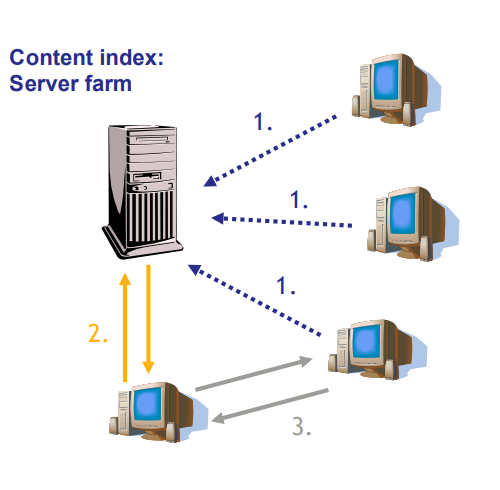
\includegraphics[scale=0.3]{figures/napster.png}
        \end{columns}
\end{frame}

\begin{frame}
    \frametitle{Napster: Discussion}
    \begin{itemize}
        \item Pros
        \begin{itemize}
            \item Consistent view of the network \\
                Central server always knows who is there and who is not.
            \item Fast and efficient searching, Search scope is O(1) \\
                Central server always knows all available files.
            \item Answer guaranteed to be corrent \\
                Nothing found means none of the current on-line peers in the network has the file.
        \end{itemize}
        \item Cons
        \begin{itemize}
            \item Single point of failure
            \item Server needs enough computation power to handle all queries
            \item Server maintains O(N) State
        \end{itemize}
    \end{itemize}
\end{frame}

\begin{frame}
    \frametitle{Gnutella: Overview}
    \begin{itemize}
        \item Napster is centralize, Gnutella is fully distributed.
        \item Based on overlay network \\
            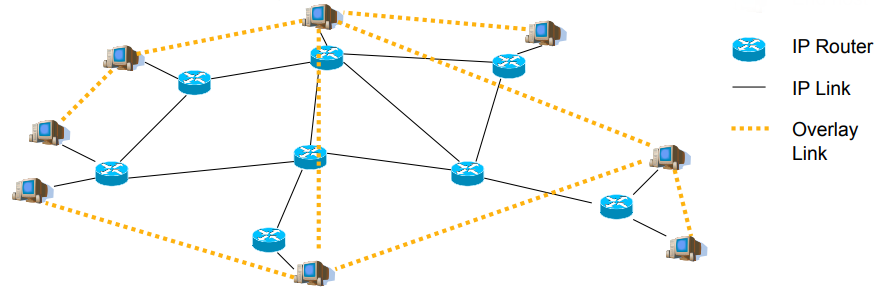
\includegraphics[scale=0.35]{figures/overlay_network.png} \\
            A virtual network on top of underlying IP network
        \item All peers are fully equal, called servents(server + client)
    \end{itemize}
\end{frame}

\begin{frame}
    \frametitle{Gnutella: Framework}
    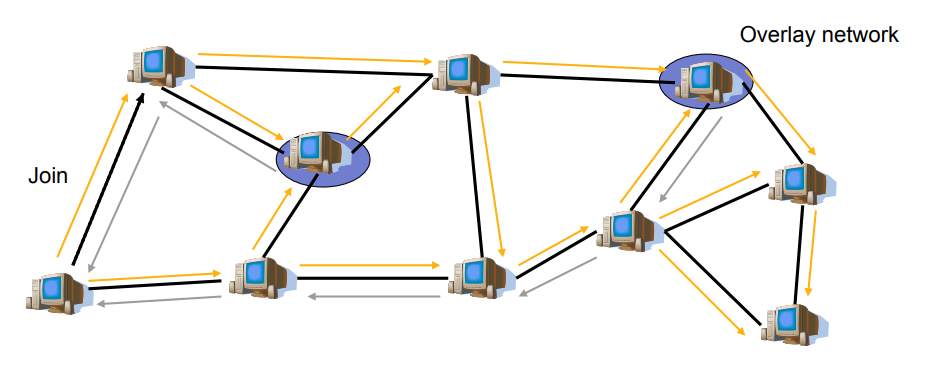
\includegraphics[scale=0.35]{figures/gnutella.png}
    \begin{itemize}
        \item To join, peer needs address of one member, learn others
        \item Queries are sent to neighbors
        \item Neighbors forword queries to their neighbors(\alert{flooding})
        \item Replies routed back via query path to querying peer
    \end{itemize}
\end{frame}

\begin{frame}
    \frametitle{Guntella: Discussion}
    \begin{itemize}
        \item Pros:
        \begin{itemize}
            \item Fully de-centralized
            \item Search cost distributed
        \end{itemize}
        \item Cons:
        \begin{itemize}
            \item Search scope is O(N)
            \item Nodes leave often, network unstable
            \item Periodic Ping/Pong consume lots of resources
        \end{itemize}
    \end{itemize}
\end{frame}

\begin{frame}
    \frametitle{KaZaA: Overview}
    \begin{itemize}
        \item Created in 2001
        \item Two kinds of nodes in KaZaA: \alert{Ordinary Nodes}, \alert{SuperNodes}
        \item ON is a normal peer run by a user
        \item SN is also a peer run by a user, but with more resources and responsibilities
        \item KaZaA forms a two-tier hierachy \\
            top level has only SN, lower level only ON
        \item ON belongs to one SN
        \item SN acts as a Napster-like hub for all its ON-children \\
            keeps track of files in those peers
    \end{itemize}
\end{frame}

\begin{frame}
    \frametitle{KaZaA: Framework}
    \begin{columns}
        \column{.5\textwidth}
        Smart Query Flooding:
        \begin{itemize}
            \item Join: on startup, client contacts a SN
            \item Publish: send list of files to SN
            \item Search: send query to SN, SN flood query amongst themselves
            \item Fetch: get the file directly from peers
        \end{itemize}
        \column{.5\textwidth}
            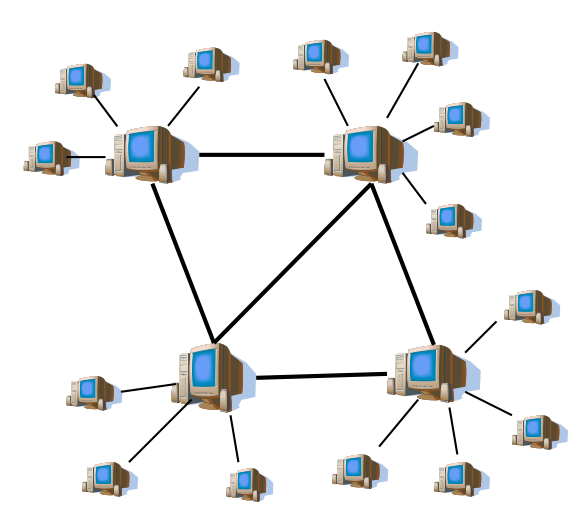
\includegraphics[scale=0.3]{figures/kazaa.png}
    \end{columns}
\end{frame}

\begin{frame}
    \frametitle{KaZaA: Discussion}
    \begin{itemize}
        \item Pros:
        \begin{itemize}
            \item Efficient searching under each SN
            \item Flooding restricted to SN only
            \item Efficient searching with 'low' resource usage
        \end{itemize}
        \item Cons:
        \begin{itemize}
            \item Still no real guarantees on search scope or search time
        \end{itemize}
    \end{itemize}
\end{frame}

\begin{frame}
    \frametitle{BitTorrent: Overview}
    2 basic ways to find objects: \\
    \begin{itemize}
        \item Search for them with keywords that match objects's description
        \item Address them using their unique name(cf. URLs in Web)
    \end{itemize}
    \begin{itemize}
        \item Swarming:
        \begin{itemize}
            \item Join: contact centralized tracker server, get a list of peers.
            \item Publish: Run a tracker server.
            \item Search: Out-of-band, E.g. use Google to find a tracker for the file you want.
            \item Fetch: Download chunks of the file from your peers. Upload chunks you have to them.
        \end{itemize}
    \end{itemize}
\end{frame}

\begin{frame}
    \frametitle{BitTorrent: Framework}
    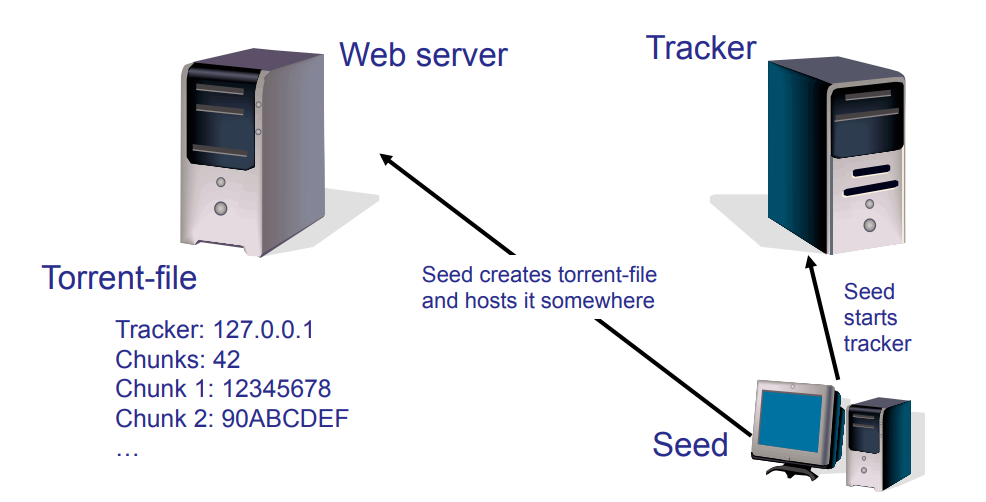
\includegraphics[scale=0.3]{figures/bittorrent.png}
\end{frame}

\begin{frame}
    \frametitle{BitTorrent: Framework}
    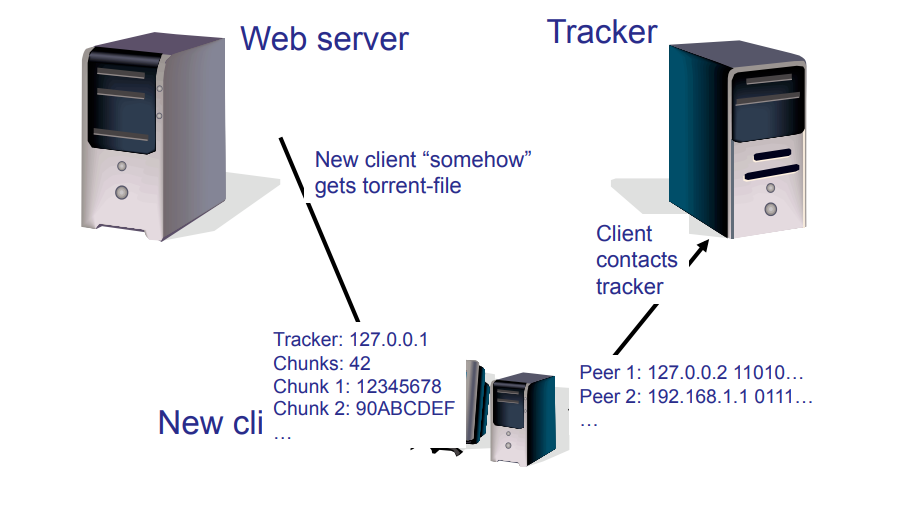
\includegraphics[scale=0.3]{figures/bittorrent2.png}
\end{frame}

\begin{frame}
    \frametitle{BitTorrent: Tit-for-Tat}
    \begin{itemize}
        \item A is downloading from some other people \\
            A will let the fastest N of those download from him.
        \item Be optimistic: occasionally let freeloaders download \\
            Otherwise no one would ever start!
    \end{itemize}
\end{frame}

\begin{frame}
    \frametitle{BitTorrent: Discussion}
    \begin{itemize}
        \item Pros:
        \begin{itemize}
            \item Works reasonably well in pratice
            \item Gives peers incentive to share resources, avoids freeriders
        \end{itemize}
        \item Cons:
        \begin{itemize}
            \item Central tracker server need to bootstrap swarm.
            \item What if tracker server fails?
        \end{itemize}
    \end{itemize}
\end{frame}

\subsection{DHT}

\begin{frame}
    \frametitle{Distributed Hash Tables}
    In BitTorrent version 4.2.0, BitTorrent introduce \alert{Trackerless} torrent using DHT.
    \begin{itemize}
        \item Actual file transfer process in P2P network is scalable \\
            File transfers directly between peers
        \item Searching does not scale in same way
        \item Put another way: Use addressing instead of searching
        \item Original motivation for DHTs: \alert{More efficient searching and object location in P2P networks}
        \item For a special resource, the tracker record the nodes/peers associated with the resource.
        \item If the tracker fails, we can \alert{lookup} the DHT for the nodes/peers info.
    \end{itemize}
\end{frame}

\begin{frame}
    \frametitle{Recall Hash Table}
    \begin{itemize}
        \item allow insertions, deletions, and lookup in constant time.
        \item fixed-size array, elements of array also called \alert{hash buckets}.
        \item Hash funtion maps keys to elements in the array.
        \item Properties of good hash functions
        \begin{itemize}
            \item Fast to compute
            \item Good distribution of keys into hash table
            \item Example: SHA-1 algorithm
        \end{itemize}
    \end{itemize}
\end{frame}

\begin{frame}
    \frametitle{DHT: Idea}
    \begin{columns}
        \column{.5\textwidth}
        \begin{itemize}
            \item Hash tables are fast for lookups.
            \item Idea: Distribute hash buckets to peers.
            \item Result is \alert{Distributed Hash Table}.
            \item Need efficient mechanism for finding which peer is responsible for which bucket and routing between them.
        \end{itemize}
        \column{.5\textwidth}
            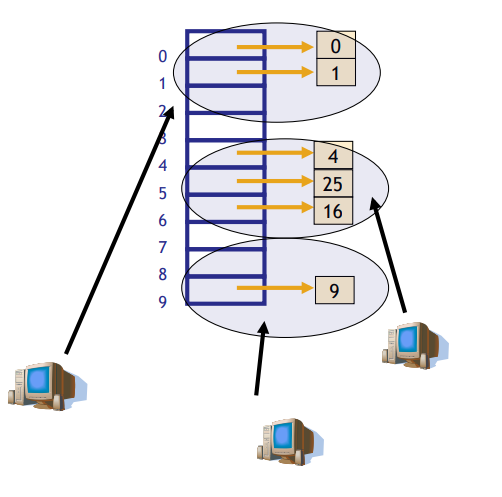
\includegraphics[scale=0.3]{figures/dht_idea.png}
    \end{columns}
\end{frame}

\begin{frame}
    \frametitle{DHT: Principle}
    \begin{columns}
        \column{.6\textwidth}
        \begin{itemize}
            \item In a DHT, each node is responsible for one or more hash buckets. \\
                As nodes join and leave, the responsibilities change.
            \item Nodes communicate among themselves to find the responsible node. \\
                Scalable Communications make DHTs efficient.
            \item Hash buckets distributed over nodes.
            \item Nodes form an \alert{overlay network}. \\
                Route messages in overlay to find responsible node.
        \end{itemize}
        \column{.4\textwidth}
            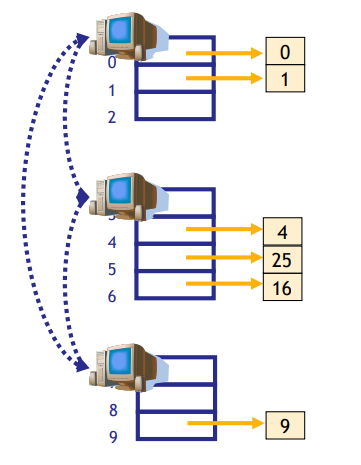
\includegraphics[scale=0.3]{figures/dht_principle.png}
    \end{columns}
\end{frame}

\begin{frame}
    \frametitle{Structured Overlay Networks/DHTs}
    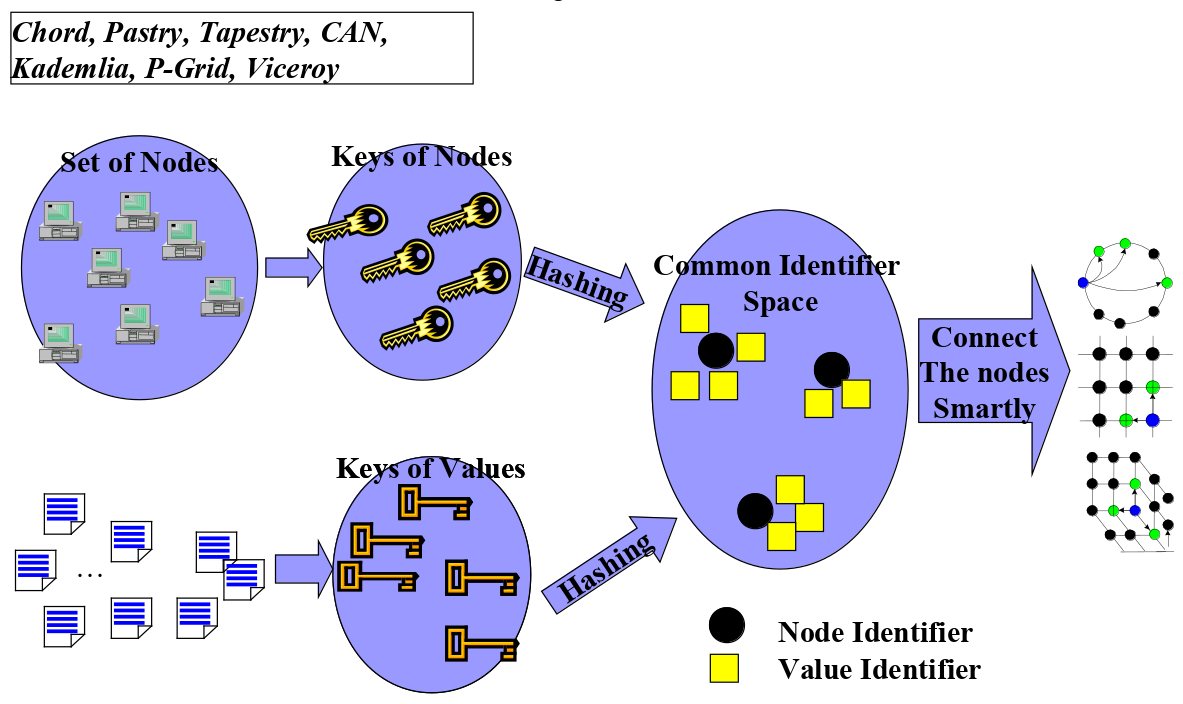
\includegraphics[scale=0.27]{figures/dht.png}
\end{frame}

\begin{frame}
    \frametitle{DHT: Overview}
    \begin{itemize}
        \item All DHTs provide the same abstraction
        \begin{itemize}
            \item Put(key, value)
            \item value = Get(key)
        \end{itemize}
        \item Difference is in overlay routing scheme
        \begin{itemize}
            \item Chord => ring
            \item Kademlia => tree
            \item CAN, Tapstry, Pastry \ldots
        \end{itemize}
    \end{itemize}
\end{frame}

\subsection{Chord}
\begin{frame}
    \frametitle{Chord: Basics}
    \begin{itemize}
        \item Chord use SHA-1 hash function
        \begin{itemize}
            \item Results in a 160-bit object/node indentifier
            \item Same hash function for obejects and nodes
        \end{itemize}
        \item Node ID hashed from IP address
        \item Object ID hashed from object name \\

        \item SHA-1 gives a 160-bit indentifier space
        \item organized in a \alert{ring} which wraps around
        \begin{itemize}
            \item Nodes keep track of \alert{predecessor} and \alert{successor}
            \item Node responsible for objects between its predecessor and itself
            \item Overlay is ofen called \alert{Chord Ring}
        \end{itemize}
    \end{itemize}
\end{frame}

\begin{frame}
    \frametitle{Node Join}
    \begin{columns}
        \column{.45\textwidth}
        \begin{itemize}
            \item Existing network with nodes on 0,1 and 4
            \item Hash of new node to join: 6
            \item Known node in network: Node 1
            \item Contact Node1
        \end{itemize}
        \column{.55\textwidth}
            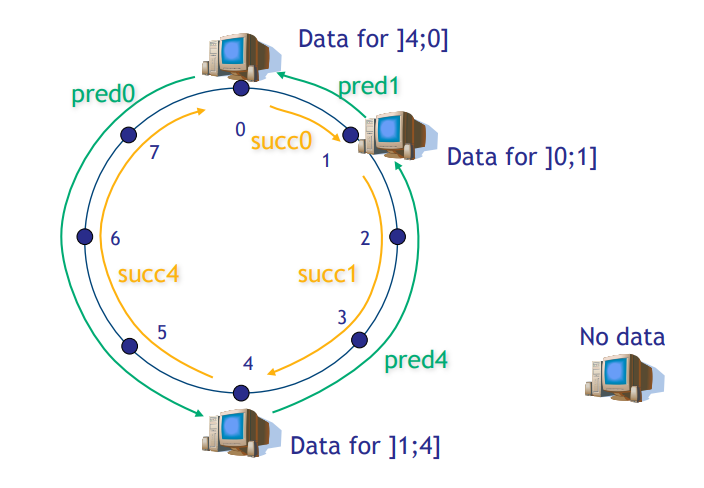
\includegraphics[scale=0.26]{figures/chord0.png}
    \end{columns}
 \end{frame}

\begin{frame}
    \frametitle{Node Join: Contact Known node}
    \begin{columns}
        \column{.45\textwidth}
        \begin{itemize}
            \item Existing network with nodes on 0,1 and 4
            \item Hash of new node to join: 6
            \item Known node in network: Node 1
            \item Contact Node1
        \end{itemize}
        \column{.55\textwidth}
            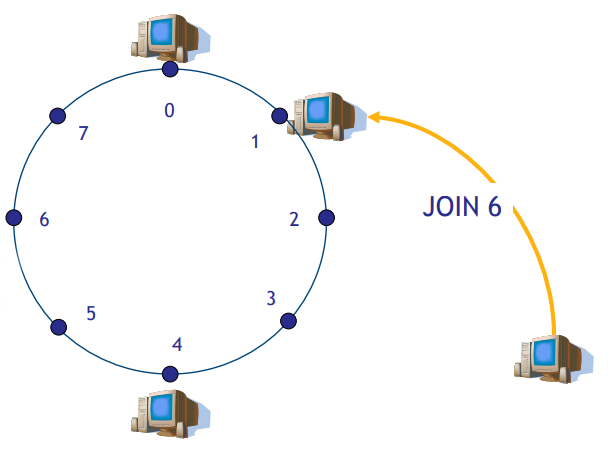
\includegraphics[scale=0.26]{figures/chord1.png}
    \end{columns}
\end{frame}

\begin{frame}
    \frametitle{Node Join: Contact Known node}
    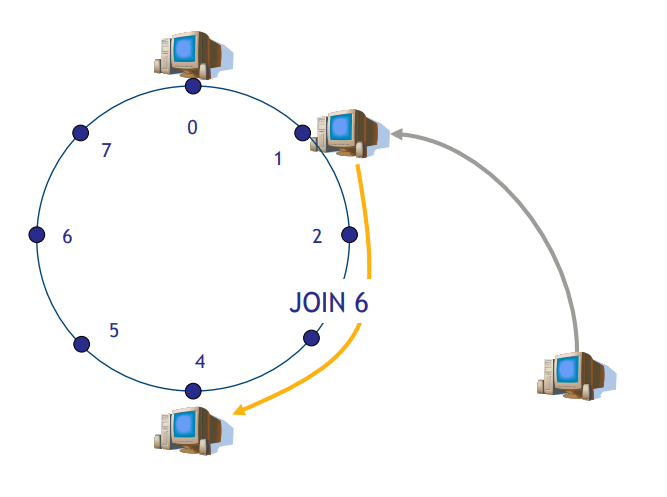
\includegraphics[scale=0.3]{figures/chord2.png}
\end{frame}

\begin{frame}
    \frametitle{Node Join: Contact Known node}
    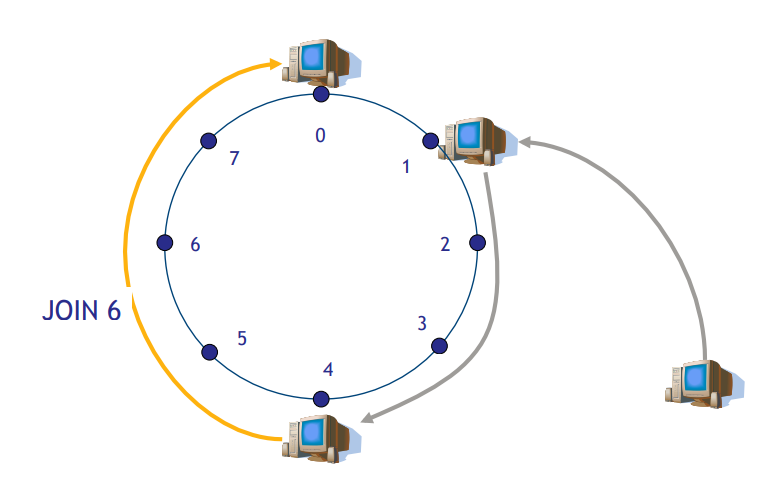
\includegraphics[scale=0.3]{figures/chord3.png}
\end{frame}

\begin{frame}
    \frametitle{Node Join: Join Successful + Transfer}
    \begin{columns}
        \column{.45\textwidth}
        \begin{itemize}
            \item Joining is successful
            \item Old responsible node transfer data that should be in new node
            \item New node informs Node4 about new successor
        \end{itemize}
        \column{.55\textwidth}
            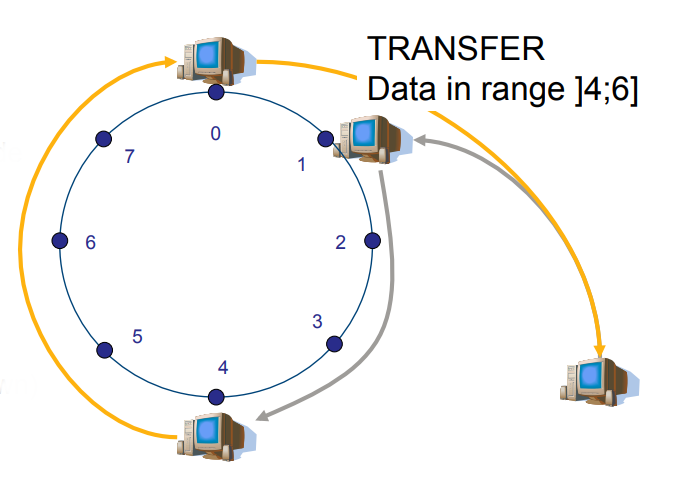
\includegraphics[scale=0.26]{figures/chord4.png}
    \end{columns}
\end{frame}

\begin{frame}
    \frametitle{Node Join: All is Done}
    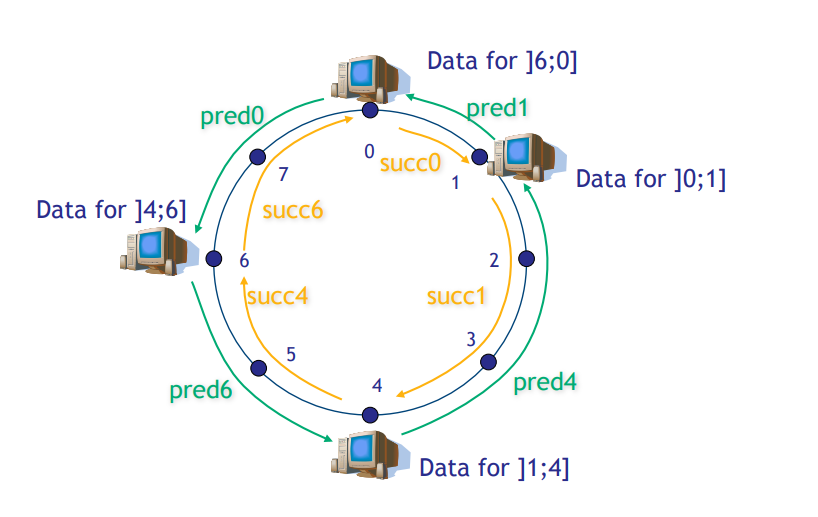
\includegraphics[scale=0.3]{figures/chord5.png}
\end{frame}

\begin{frame}
    \frametitle{Storing a Value}
    \begin{columns}
        \column{.45\textwidth}
        \begin{itemize}
            \item Node6 wants to strore object with name 'FOO' and value 5
            \item hash(Foo) = 2
        \end{itemize}
        \column{.55\textwidth}
            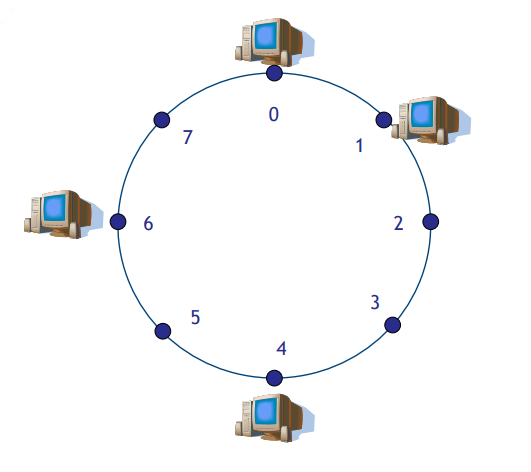
\includegraphics[scale=0.26]{figures/chord6.png}
    \end{columns}
\end{frame}

\begin{frame}
    \frametitle{Storing a Value}
    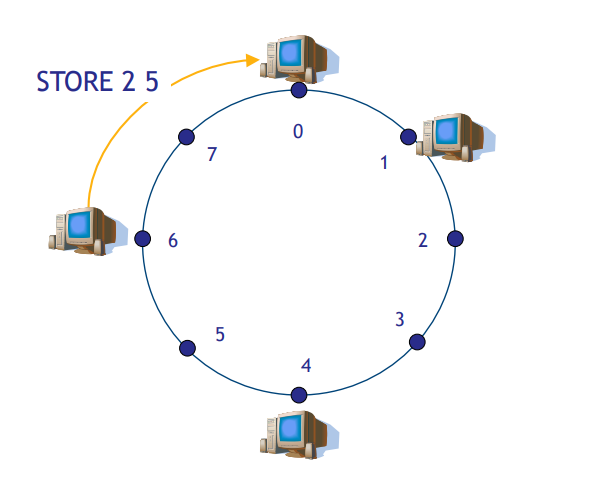
\includegraphics[scale=0.3]{figures/chord7.png}
\end{frame}

\begin{frame}
    \frametitle{Storing a Value}
    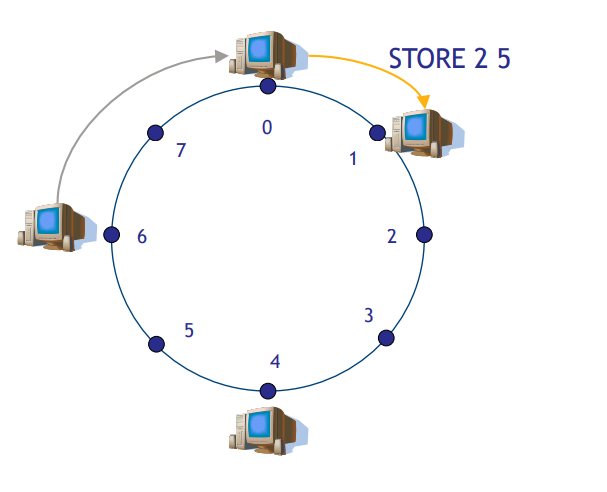
\includegraphics[scale=0.3]{figures/chord8.png}
\end{frame}

\begin{frame}
    \frametitle{Storing a Value}
    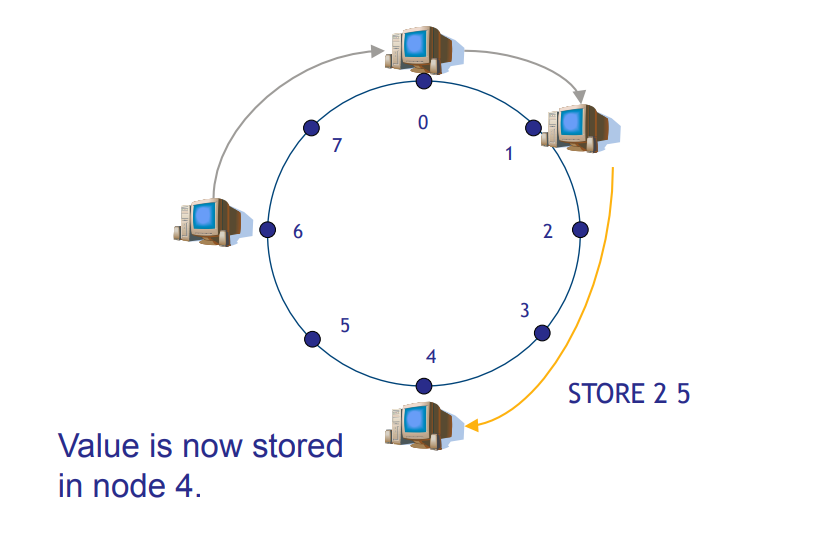
\includegraphics[scale=0.3]{figures/chord9.png}
\end{frame}

\begin{frame}
    \frametitle{Retrieving a Value}
    \begin{columns}
        \column{.45\textwidth}
        \begin{itemize}
            \item Node1 wants to get object with name 'FOO'
            \item hash(Foo) = 2
            \item Foo is stored on Node4
        \end{itemize}
        \column{.55\textwidth}
            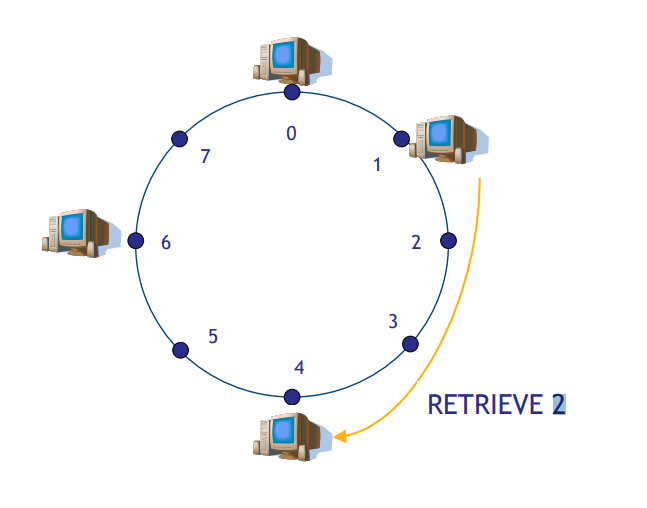
\includegraphics[scale=0.26]{figures/chord10.png}
    \end{columns}
\end{frame}

\begin{frame}
    \frametitle{Retrieving a Value}
    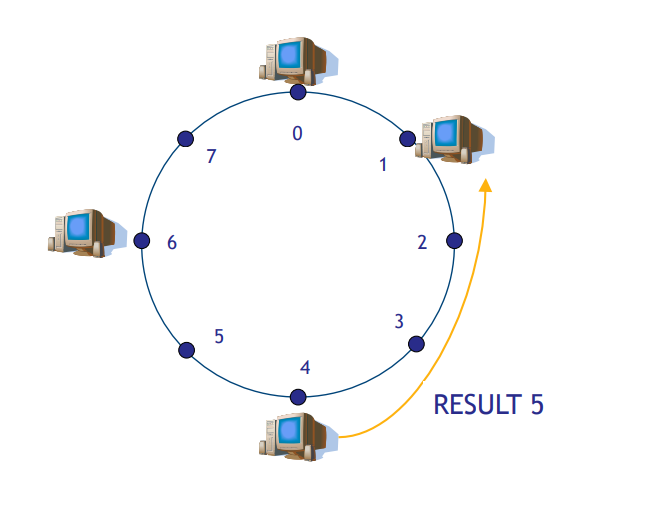
\includegraphics[scale=0.3]{figures/chord11.png}
\end{frame}

\begin{frame}
    \frametitle{Scalable Key Location: Finger Tables}
    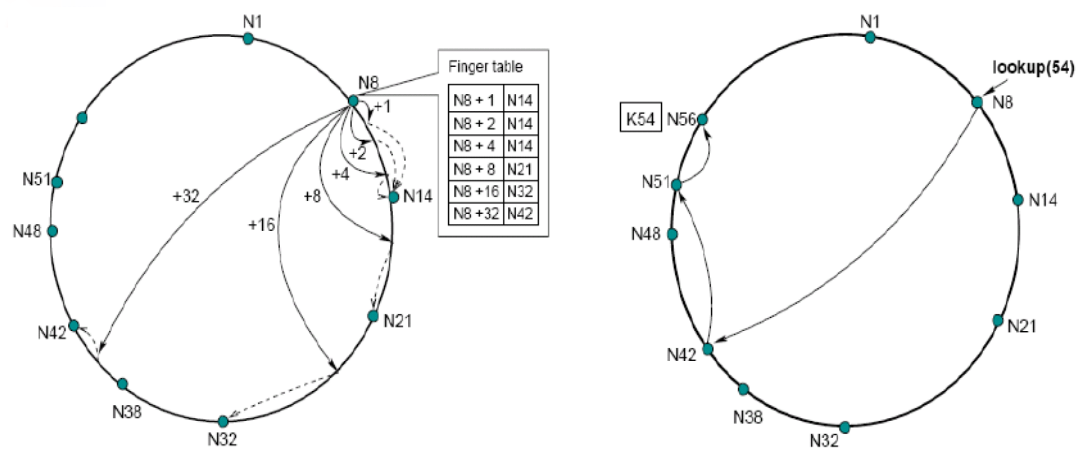
\includegraphics[scale=0.3]{figures/fingertable1.png} \\
    Row i in finger table at node n contains first node s that succeeds n by least $2^{i-1}$ on the ring. First finger is the successor.
\end{frame}

\begin{frame}
    P2P system ends here. \\
    Let's go back to distributed system.
\end{frame}
